%%%% Elementos pós-textuais
%%
%% Glossário, apêndices, anexos e índice remissivo (opcionais).

%% Apêndices
\begin{Appendix}

    \section{APÊNDICE A — MODELO DE NEGÓCIOS CANVAS}%
    \label{sect:apx-a1}
    
    \begin{figure}[H]
    \centering
    \caption{Figura A.1 -  Modelo de negócios Canvas}%
    \label{fig:canvaspi}
    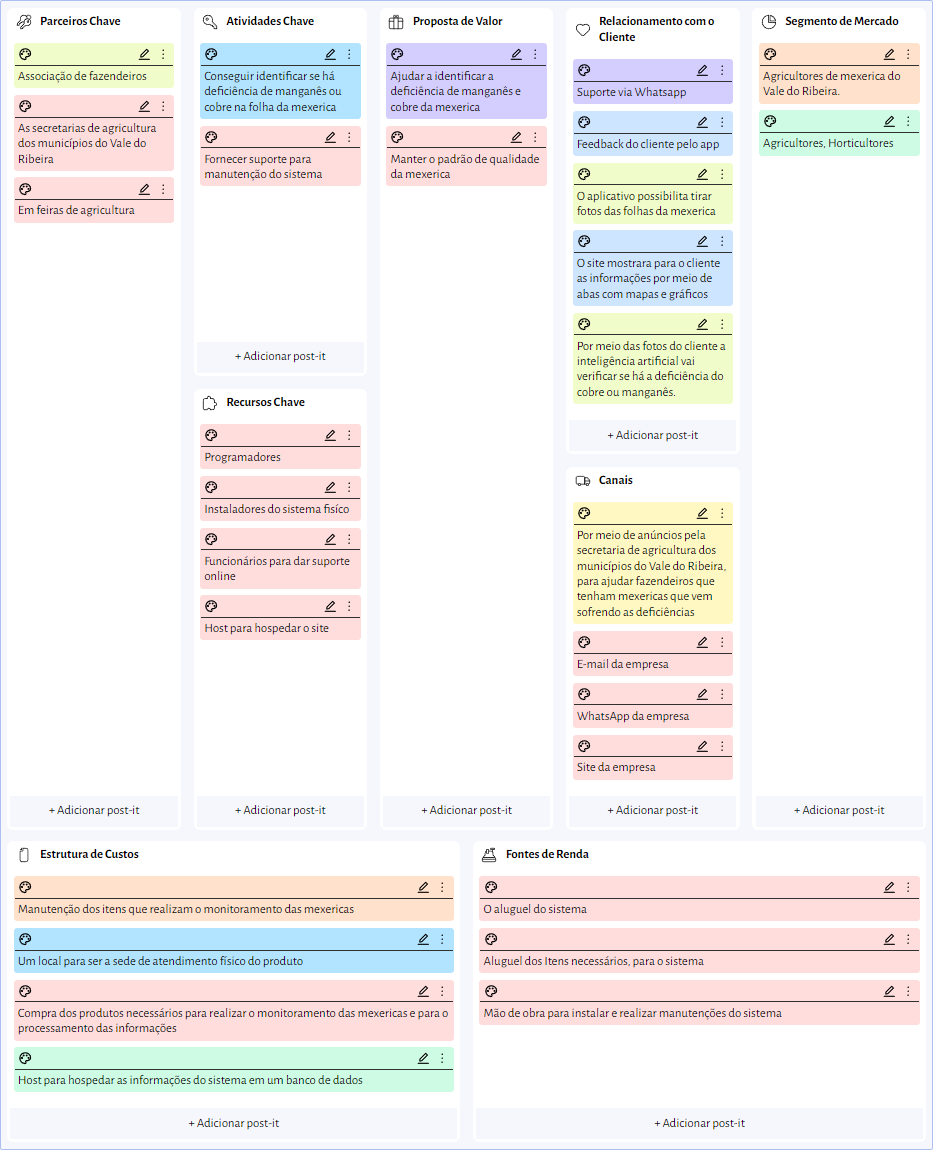
\includegraphics[width=0.8\linewidth]{Illustrations/canvas.png}
    \SourceOrNote{Autoria Própria (2025)}
    \end{figure}

    \section{APÊNDICE B — FLUXOGRAMA  DO MÉTODO DESENVOLVIDO}%
    \label{sect:apx-b1}

    \begin{figure}[H]
    \centering
    \caption{Figura B.1 -  Fluxograma do método de diagnóstico automatizado baseado em visão computacional}%
    \label{fig:fluxograma-metodo}
    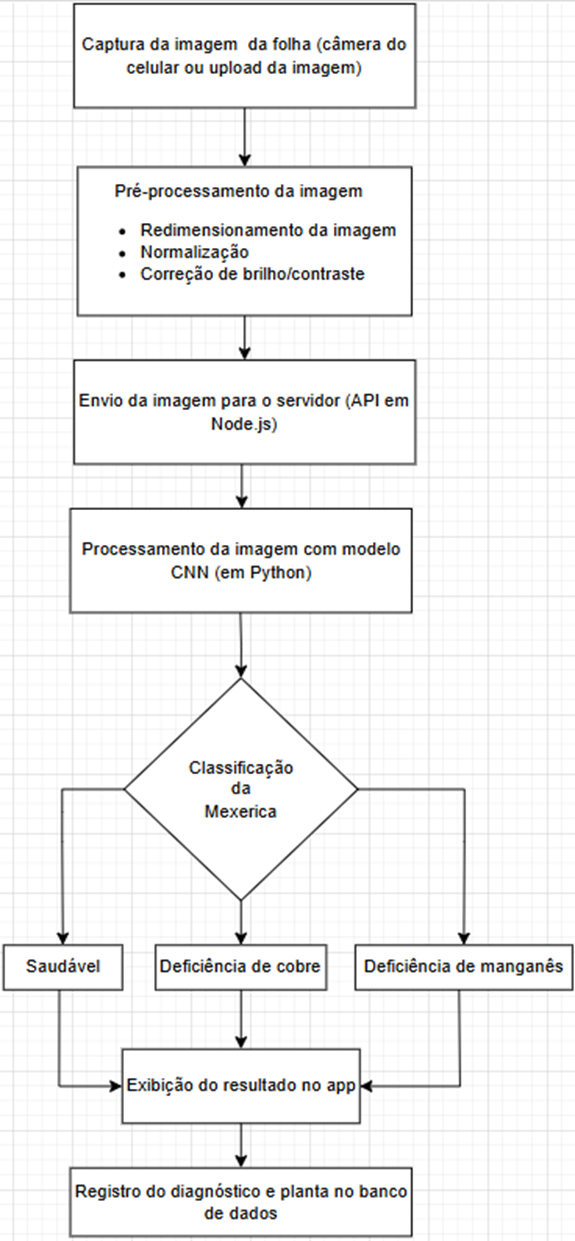
\includegraphics[width=0.4\linewidth]{Illustrations/fluxograma1.png}
    \SourceOrNote{Autoria Própria (2025)}
    \end{figure}
    
\end{Appendix}
    
    
    %% Índice remissivo
\printindex%
    